\documentclass{beamer}
	% Clears navigation bar and symbols
	\setbeamertemplate{footline}[page number]{}
	\setbeamertemplate{navigation symbols}{}
	\usetheme{Copenhagen}

	\usepackage{graphicx}
	\usepackage{amsmath}
	\usepackage{amsthm}

	\newtheorem{thm}{Theorem}
	\newtheorem{prop}{Proposition}

	\usepackage{tikz}
	\usepackage{tikz-uml}
	\usepackage{xcolor}

	\tikzstyle{node} = [draw, circle, node distance=0.5]
	\tikzstyle{edgenode} =[rectangle, midway, fill=white, font=\color{black!50}\tiny]
	\tikzstyle{line} = [draw, thick]
	\tikzstyle{vec} = [draw, ->, -latex, ultra thick, orange]

	\author{Gio Borje and Craig Steinke}
	\institute{UC Irvine}
	\title{High-Level Sprout Geometry Extraction and Analysis of In Vitro Angiogenesis}
	\date{July 23, 2013}
% \setbeamercovered{transparent}
\begin{document}

\begin{frame}
	\maketitle
\end{frame}

\begin{frame}{Overview}
	\begin{columns}
	\begin{column}{0.5\textwidth}
		\begin{figure}
			\centering
			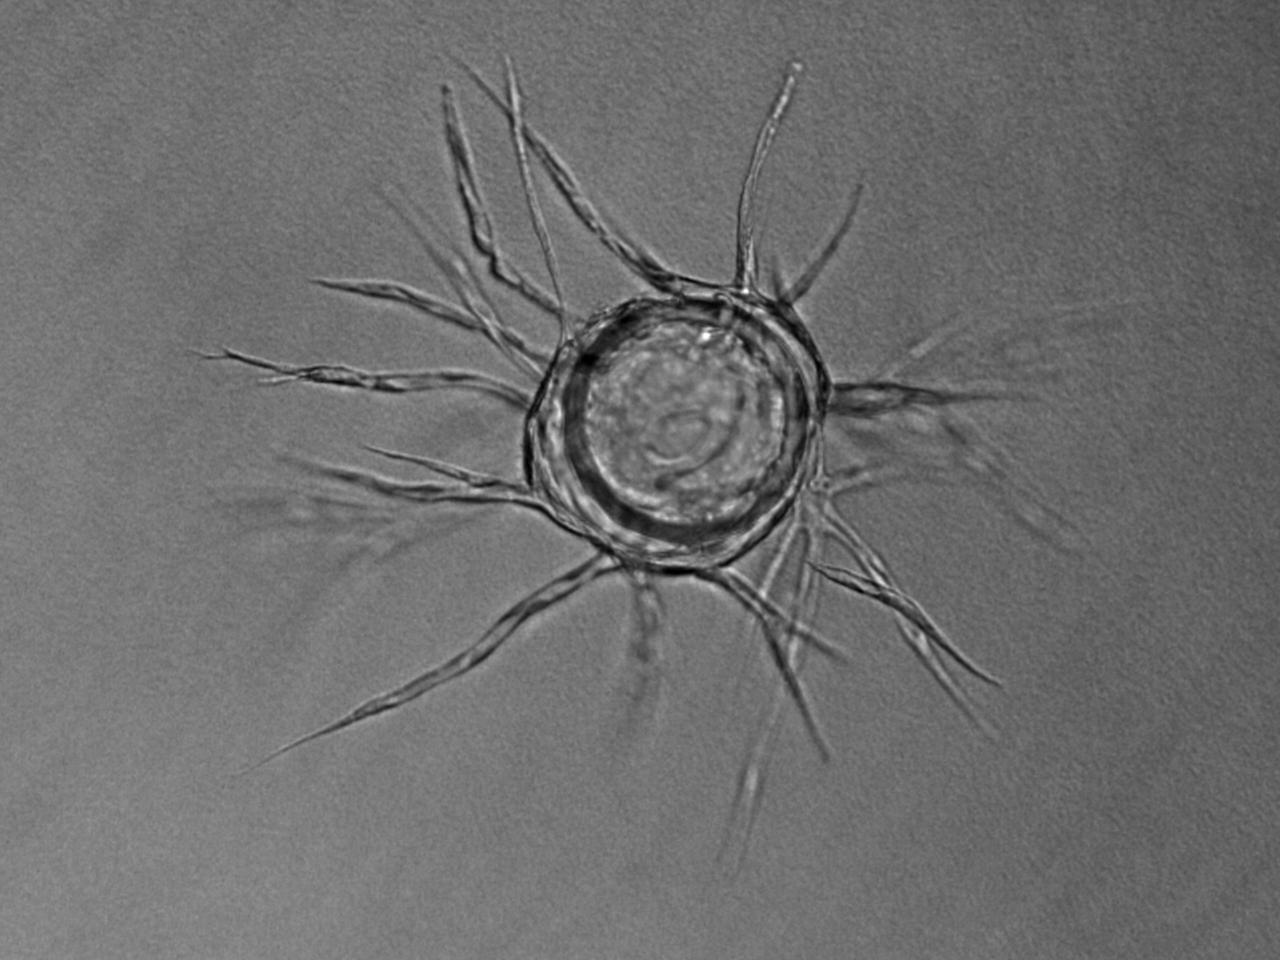
\includegraphics[width=\textwidth]{images/mono}
			\caption{Before}
		\end{figure}
	\end{column}
	\begin{column}{0.5\textwidth}
		\begin{figure}
			\centering
			\begin{tabular}{|l|}
				\hline
				\textbf{Spreadsheet Report} \\\hline
				Sprout Counts \\\hline
				$\vdots$ \\\hline
				Branching Factor \\\hline
			\end{tabular}
			\caption{After}
		\end{figure}
	\end{column}
	\end{columns}
\end{frame}

\begin{frame}{Outline}
	\begin{enumerate}
		\item Motivation
		\item Fibrin Gel Bead Sprouting Assay (FGBSA)
		\item Methodology
		\item Results
	\end{enumerate}
\end{frame}

\begin{frame}{Motivation}
	Solid tumors have an avascular (no nearby blood vessels) growth phase
	that allows for an approximate maximum size of 1-2mm in
	diameter\footnote{Robert S. Kerbel. Tumor angiogenesis: past, present
	and the near future. \emph{Carcinogenesis}, 21(3):505–515, 1999.}.

	\pause
	\vspace{2em}
	Think of the size of \emph{very coarse sand}.
	
	\pause
	\vspace{2em}
	Tumor angiogesesis enables relentless tumor growth and metastasis.
\end{frame}

\begin{frame}{FGBSA Image}
	\begin{figure}
		\centering
		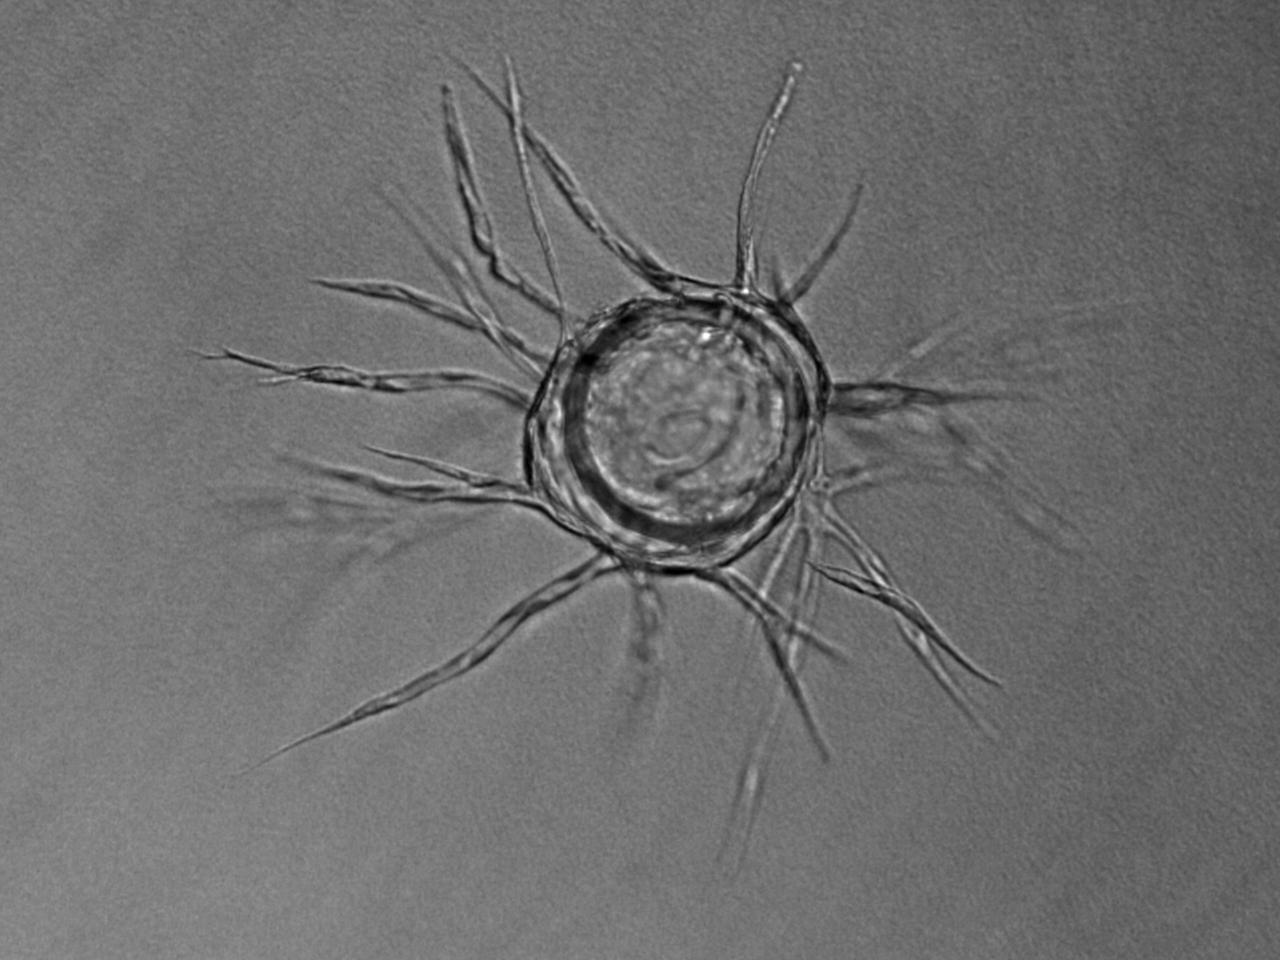
\includegraphics[width=\textwidth]{images/mono}
	\end{figure}
\end{frame}

\begin{frame}{Current Methodology}
	\begin{enumerate}
		\item Sprout Restoration
		\item Sholl Analysis
	\end{enumerate}
\end{frame}

\begin{frame}{Current Methodology}
	\begin{enumerate}
		\item Edge Detection and Polygon Approximation
		\item Bead Detection (Hough Transform)
		\item Non-Sprout Detection
		\item Dilation for Approximate Centerline
		\item Thinning and Pruning
		\item \textbf{Sholl Analysis}
	\end{enumerate}

	Expanded sprout restoration methods
\end{frame}

\begin{frame}{Original Image}
	\begin{figure}
		\centering
		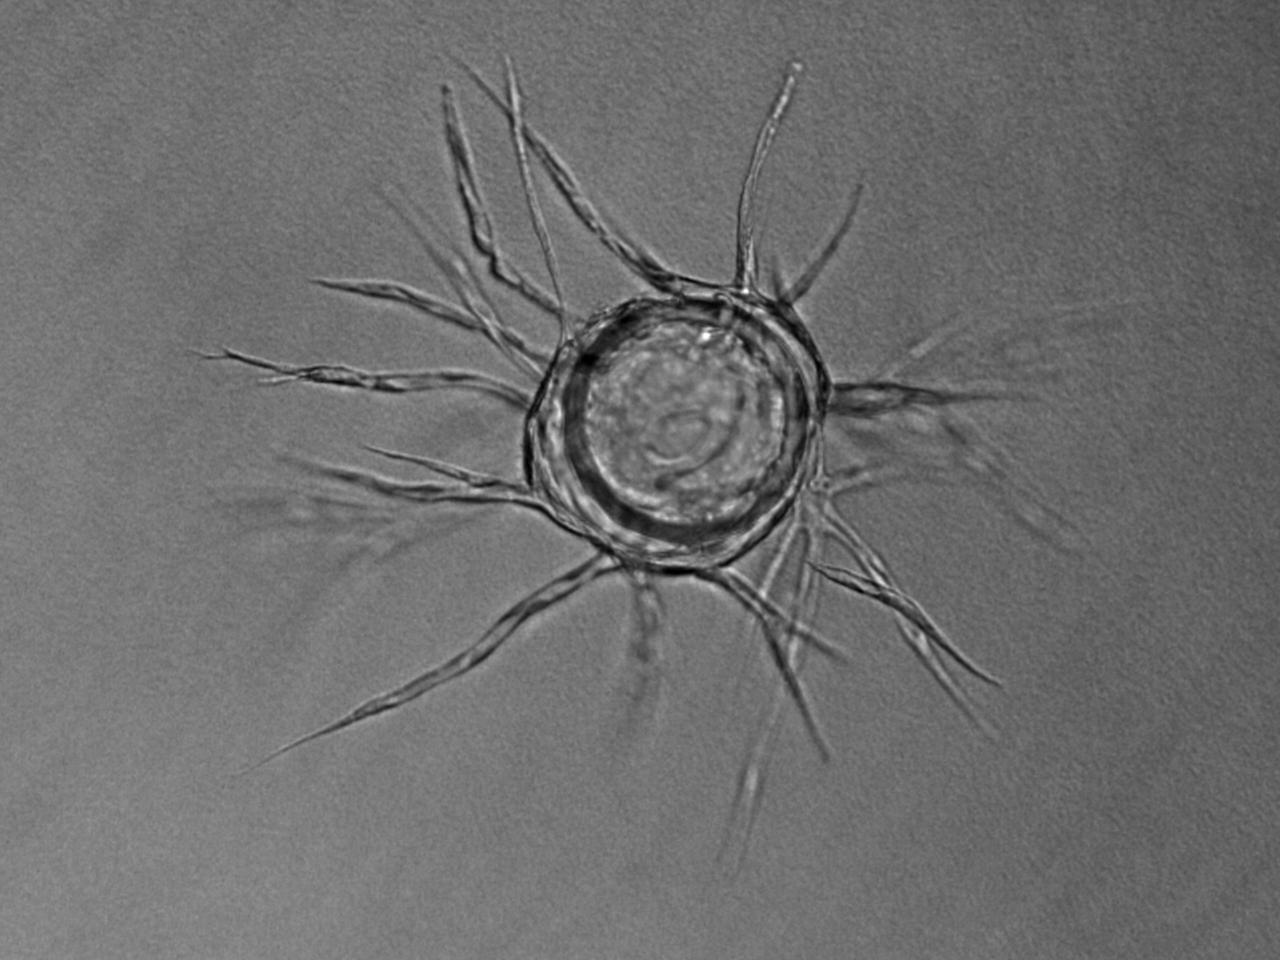
\includegraphics[width=\textwidth]{images/mono}
	\end{figure}
\end{frame}

\begin{frame}{Edge Detection and Polygon Approximation}
	\begin{figure}
		\centering
		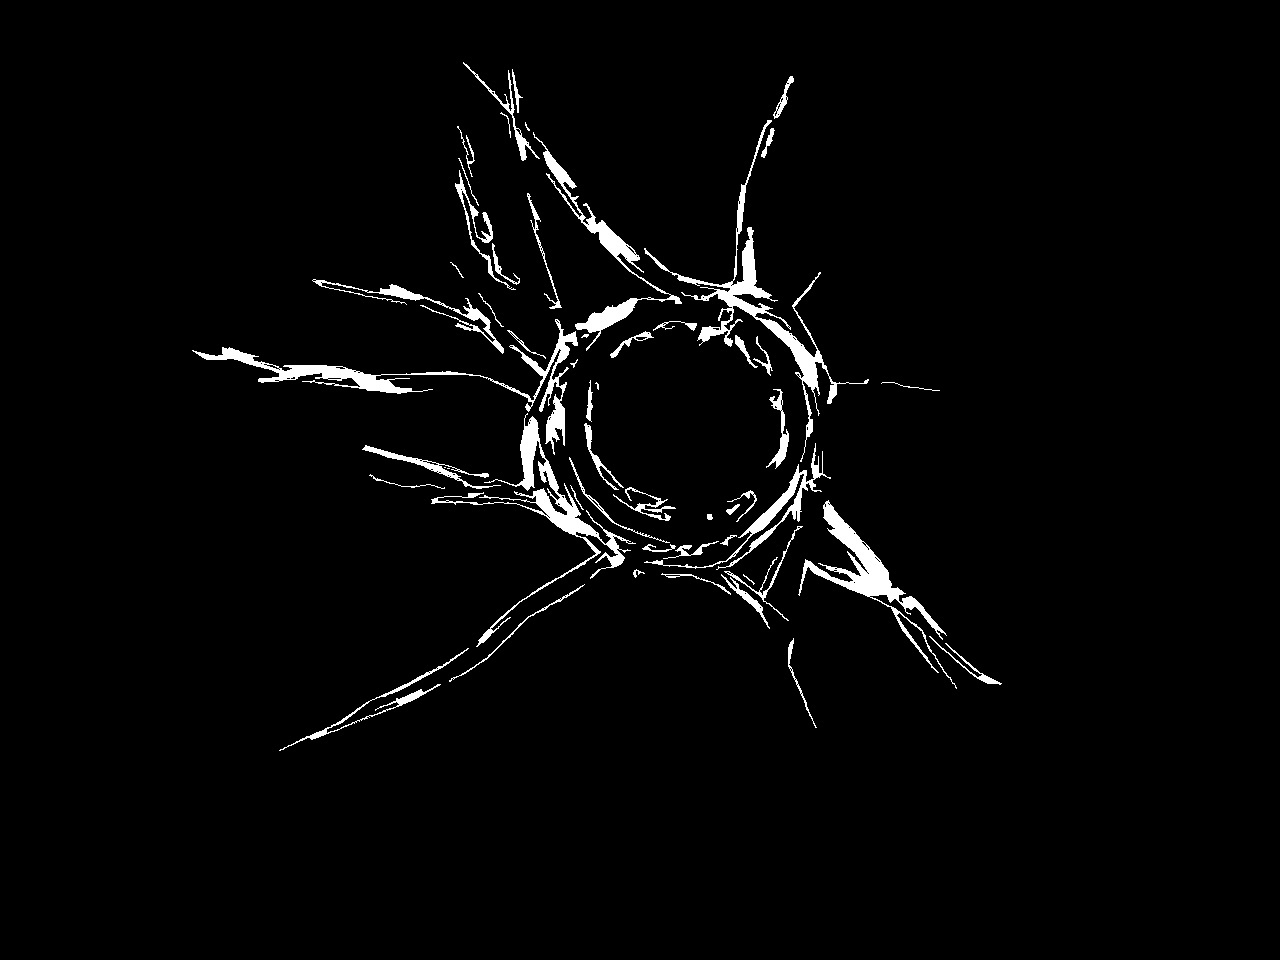
\includegraphics[width=\textwidth]{images/mono_preprocessed}
	\end{figure}
\end{frame}

\begin{frame}{Bead Detection (Hough Transform)}
	\begin{figure}
		\centering
		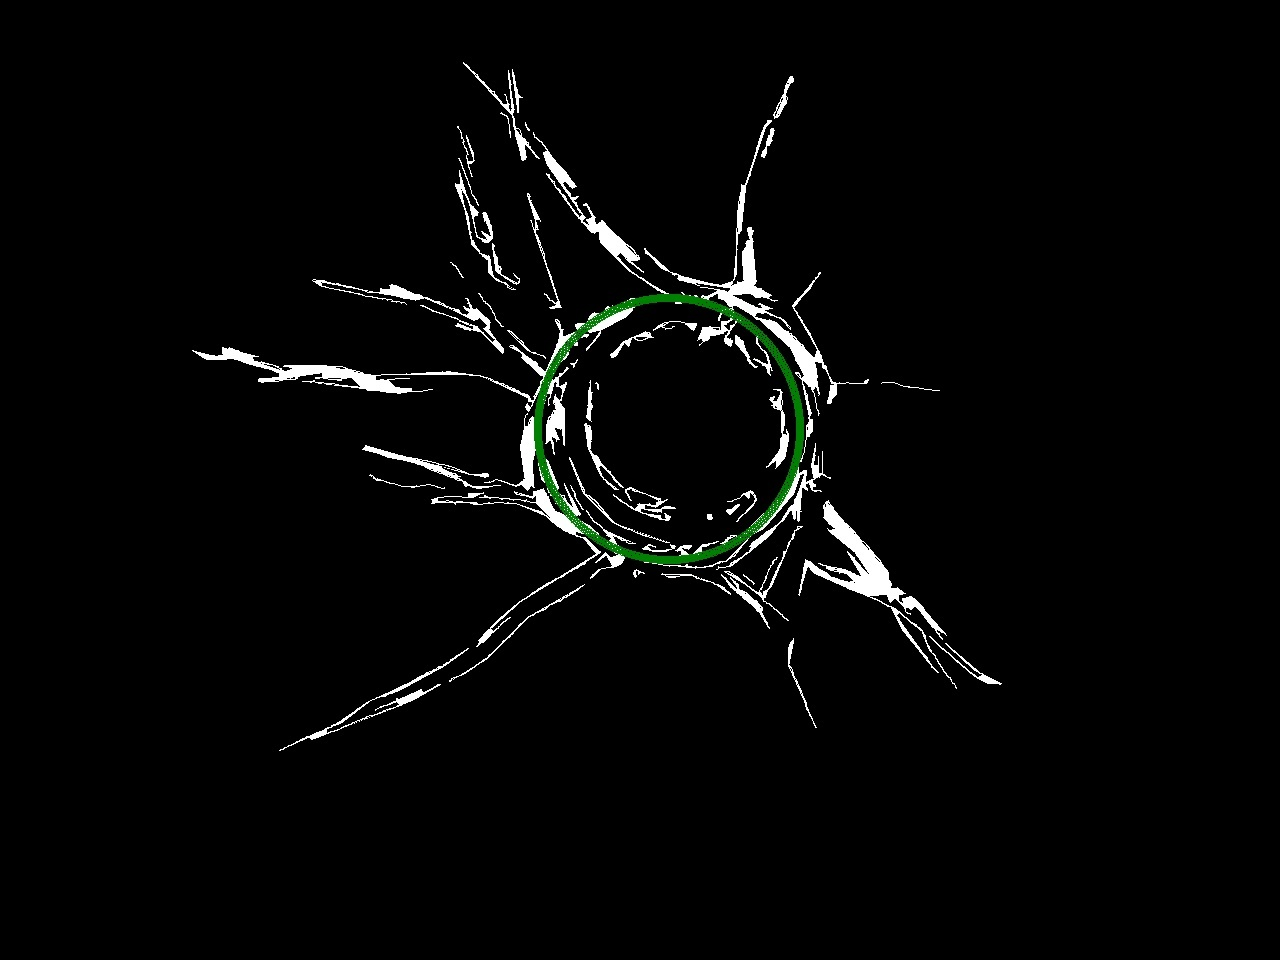
\includegraphics[width=\textwidth]{images/mono_found_circle}
	\end{figure}
\end{frame}

\begin{frame}{Dilation for Approximate Centerline}
	\begin{figure}
		\centering
		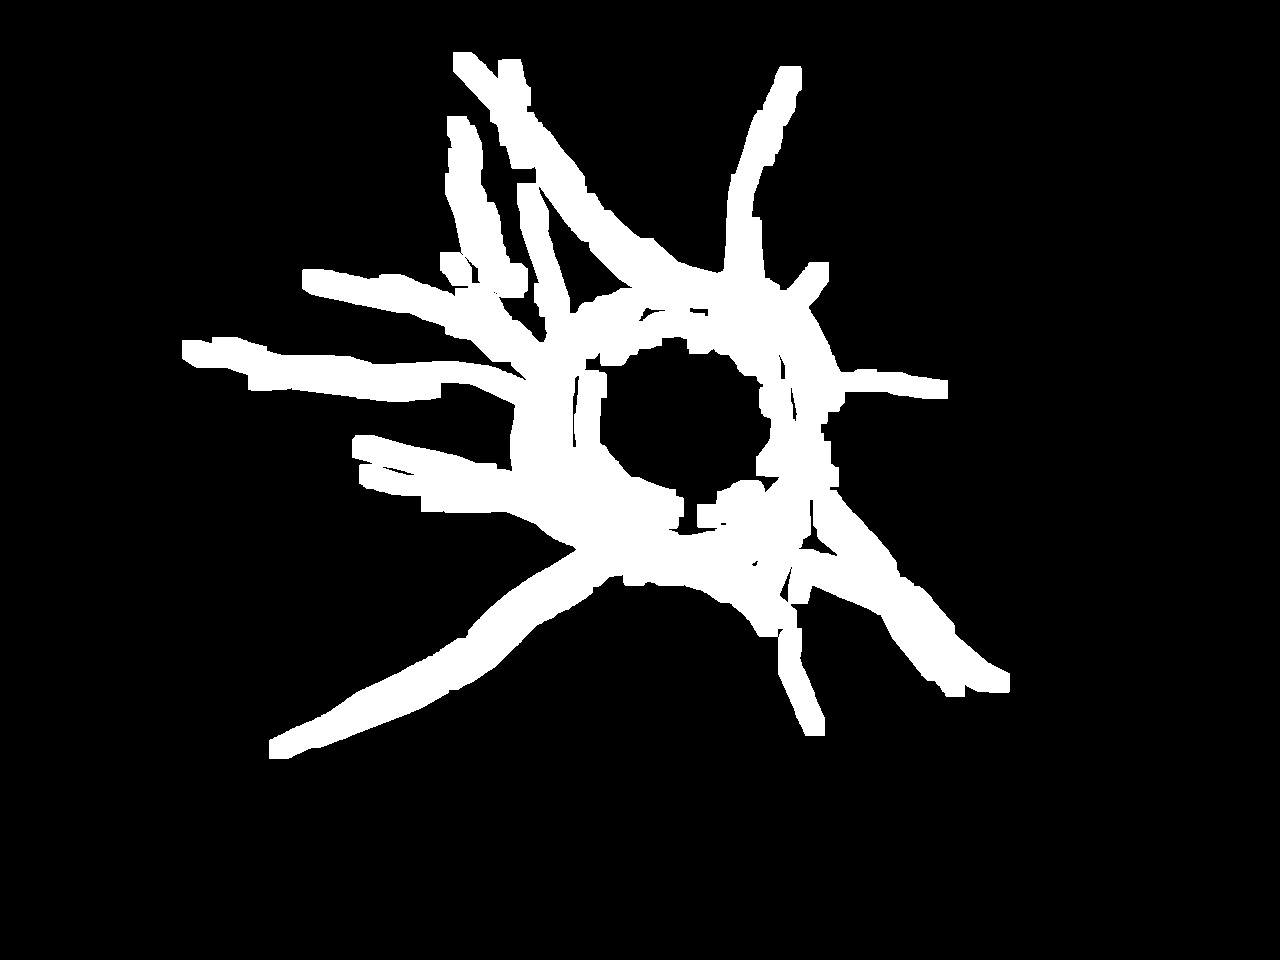
\includegraphics[width=\textwidth]{images/mono_dilated}
	\end{figure}
\end{frame}

\begin{frame}{Thinning and Pruning}
	\begin{figure}
		\centering
		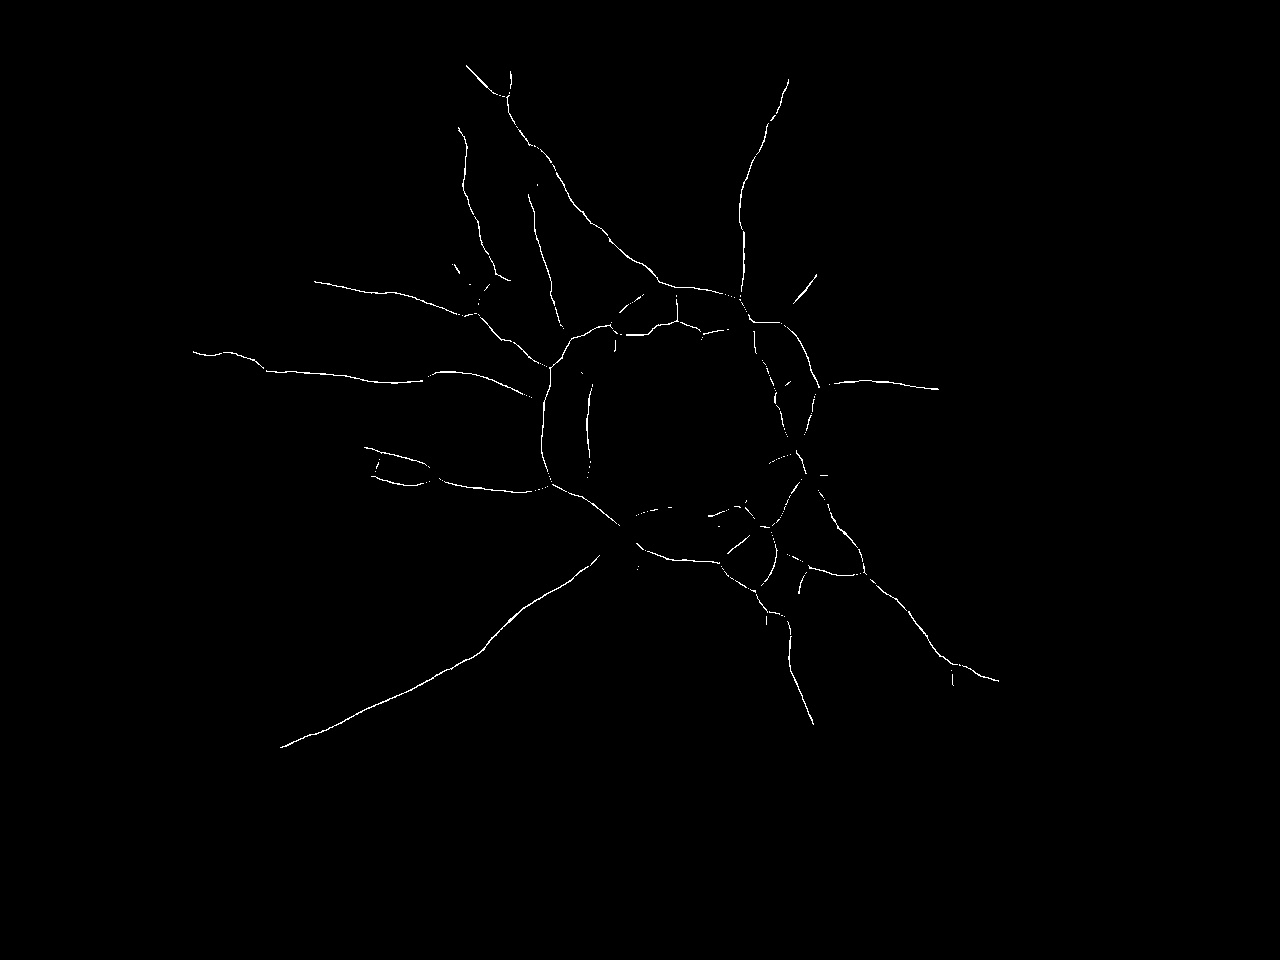
\includegraphics[width=\textwidth]{images/mono_skeletonized}
	\end{figure}
\end{frame}

\begin{frame}{Sholl Analysis: Why}
	\begin{columns}
		\begin{column}{0.6\textwidth}
		\begin{figure}
			\centering
			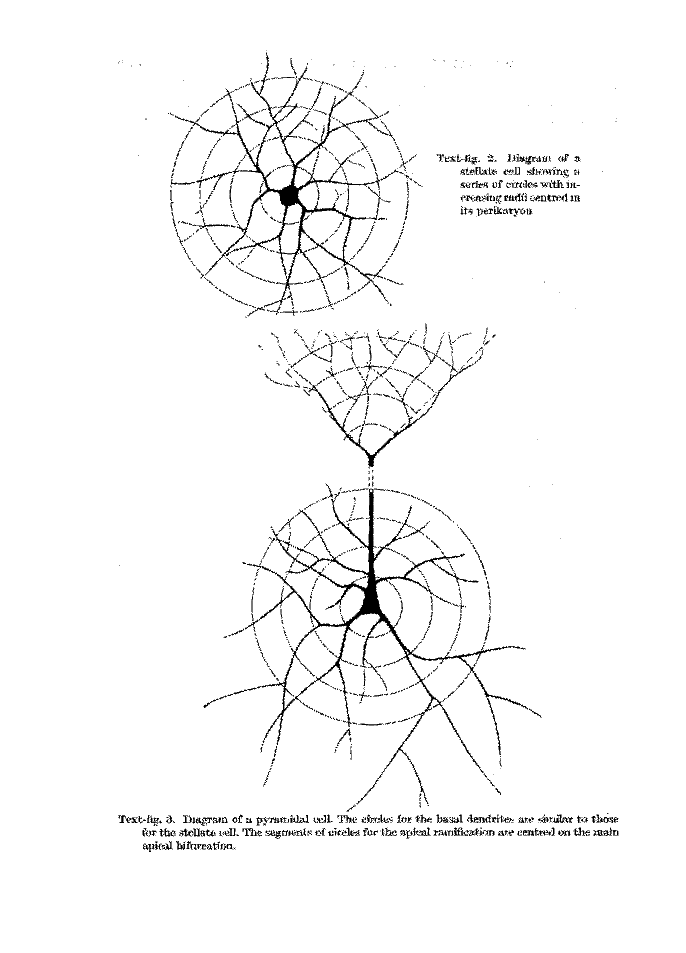
\includegraphics[height=0.6\textheight]{sholl}
			\caption{ D. A. Sholl. Dendritic organization in the neurons of
				the visual and motor cortices of the cat. \emph{J Anat.},
				87(4):387–406, 1953.  }
		\end{figure}
		\end{column}
		\begin{column}{0.4\textwidth}
		\begin{itemize}
			\item No tracing required
			\item Morphometric descriptors can be obtained
		\end{itemize}
		\end{column}
	\end{columns}
\end{frame}

\begin{frame}{Sholl Analysis: Implementation}
	\begin{figure}[h]
		\centering
		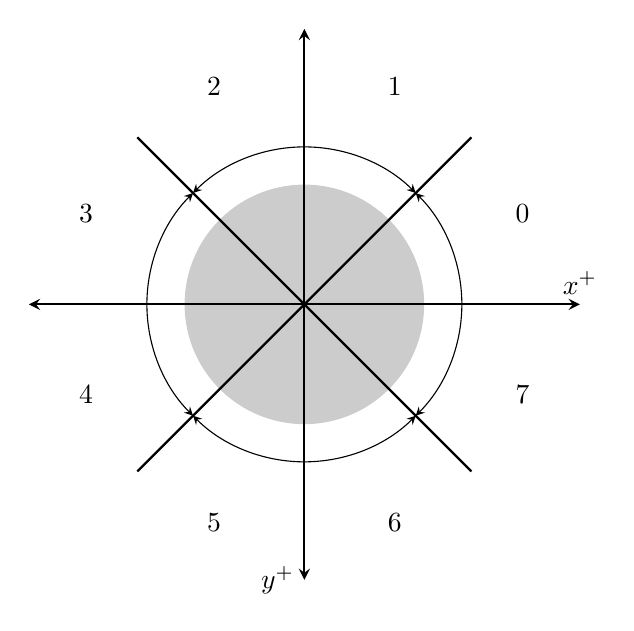
\begin{tikzpicture}[>=stealth]
			\draw [very thick, color=black!20, fill] (0,0) circle (1.5);

			%% Coordinate axes
			\draw [<->,thick] (-3.5,0) -- (3.5,0) node [above] {$x^+$};
			\draw [<->,thick] (0,3.5) -- (0,-3.5) node [left] {$y^+$};

			%% Diagonals
			\draw [thick] (0,0) +(45:-3) -- (45:3);
			\draw [thick] (0,0) +(135:-3) -- (135:3);

			%% Even arcs
			\foreach \x in {0,1,2,3} {
				\pgfmathmultiply{\x}{90}
				\pgfmathtruncatemacro{\alpha}{\pgfmathresult}
				\draw [->] (0,0) +(0+\alpha:2cm) arc (0+\alpha:45+\alpha:2cm);
				\pgfmathmultiply{\x}{2}
				\pgfmathtruncatemacro{\arclabel}{\pgfmathresult}
				\path (0,0) +(22.5+\alpha:3cm) node {$\arclabel$};
			}

			%% Odd arcs
			\foreach \x in {0,1,2,3} {
				\pgfmathmultiply{\x}{90}
				\pgfmathtruncatemacro{\alpha}{\pgfmathresult}
				\draw [->] (0,0) +(90+\alpha:2cm) arc (90+\alpha:90+\alpha-45:2cm);
				\pgfmathparse{2*\x+1}
				\pgfmathtruncatemacro{\arclabel}{\pgfmathresult}
				\path (0,0) +(67.5+\alpha:3cm) node {$\arclabel$};
			}
		\end{tikzpicture}
	\end{figure}
\end{frame}

\begin{frame}{Sholl Analysis: Bresenham Circle Algorithm}
	\begin{figure}[h]
		\centering
		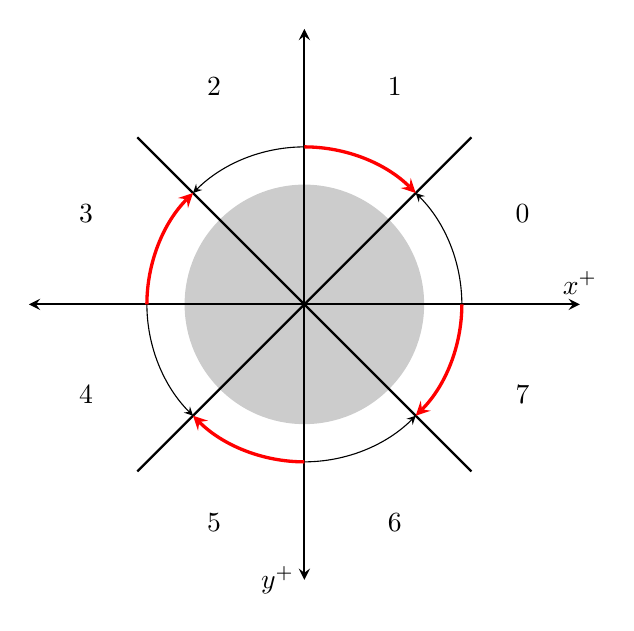
\begin{tikzpicture}[>=stealth]
			\draw [very thick, color=black!20, fill] (0,0) circle (1.5);

			%% Coordinate axes
			\draw [<->,thick] (-3.5,0) -- (3.5,0) node [above] {$x^+$};
			\draw [<->,thick] (0,3.5) -- (0,-3.5) node [left] {$y^+$};

			%% Diagonals
			\draw [thick] (0,0) +(45:-3) -- (45:3);
			\draw [thick] (0,0) +(135:-3) -- (135:3);

			%% Even arcs
			\foreach \x in {0,1,2,3} {
				\pgfmathmultiply{\x}{90}
				\pgfmathtruncatemacro{\alpha}{\pgfmathresult}
				\draw [->] (0,0) +(0+\alpha:2cm) arc (0+\alpha:45+\alpha:2cm);
				\pgfmathmultiply{\x}{2}
				\pgfmathtruncatemacro{\arclabel}{\pgfmathresult}
				\path (0,0) +(22.5+\alpha:3cm) node {$\arclabel$};
			}

			%% Odd arcs
			\foreach \x in {0,1,2,3} {
				\pgfmathmultiply{\x}{90}
				\pgfmathtruncatemacro{\alpha}{\pgfmathresult}
				\draw [->, color=red, very thick] (0,0) +(90+\alpha:2cm) arc (90+\alpha:90+\alpha-45:2cm);
				\pgfmathparse{2*\x+1}
				\pgfmathtruncatemacro{\arclabel}{\pgfmathresult}
				\path (0,0) +(67.5+\alpha:3cm) node {$\arclabel$};
			}
		\end{tikzpicture}
	\end{figure}
\end{frame}

\begin{frame}{Sholl Analysis: Unordered Property of Circle Algorithm}
	\begin{figure}[h]
		\centering
		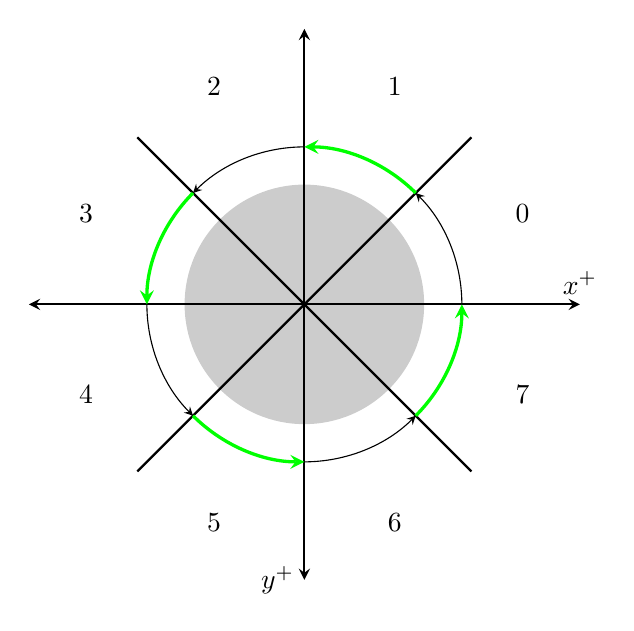
\begin{tikzpicture}[>=stealth]
			\draw [very thick, color=black!20, fill] (0,0) circle (1.5);

			%% Coordinate axes
			\draw [<->,thick] (-3.5,0) -- (3.5,0) node [above] {$x^+$};
			\draw [<->,thick] (0,3.5) -- (0,-3.5) node [left] {$y^+$};

			%% Diagonals
			\draw [thick] (0,0) +(45:-3) -- (45:3);
			\draw [thick] (0,0) +(135:-3) -- (135:3);

			%% Even arcs
			\foreach \x in {0,1,2,3} {
				\pgfmathmultiply{\x}{90}
				\pgfmathtruncatemacro{\alpha}{\pgfmathresult}
				\draw [->] (0,0) +(0+\alpha:2cm) arc (0+\alpha:45+\alpha:2cm);
				\pgfmathmultiply{\x}{2}
				\pgfmathtruncatemacro{\arclabel}{\pgfmathresult}
				\path (0,0) +(22.5+\alpha:3cm) node {$\arclabel$};
			}

			%% Odd arcs
			\foreach \x in {0,1,2,3} {
				\pgfmathmultiply{\x}{90}
				\pgfmathtruncatemacro{\alpha}{\pgfmathresult}
				\draw [<-, color=green, very thick] (0,0) +(90+\alpha:2cm) arc (90+\alpha:90+\alpha-45:2cm);
				\pgfmathparse{2*\x+1}
				\pgfmathtruncatemacro{\arclabel}{\pgfmathresult}
				\path (0,0) +(67.5+\alpha:3cm) node {$\arclabel$};
			}
		\end{tikzpicture}
	\end{figure}
\end{frame}

\begin{frame}{Sholl Analysis: Ordered Bresenham Circle Algorithm}
	\begin{figure}[h]
		\centering
		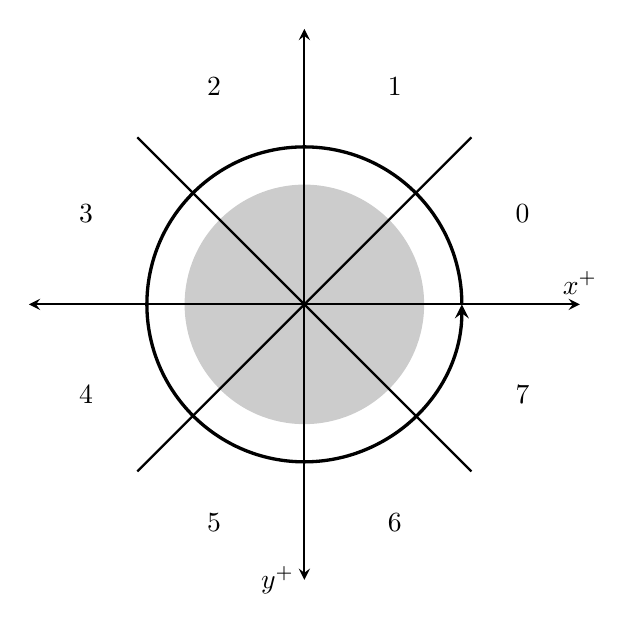
\begin{tikzpicture}[>=stealth]
			\draw [very thick, color=black!20, fill] (0,0) circle (1.5);

			%% Coordinate axes
			\draw [<->,thick] (-3.5,0) -- (3.5,0) node [above] {$x^+$};
			\draw [<->,thick] (0,3.5) -- (0,-3.5) node [left] {$y^+$};

			%% Diagonals
			\draw [thick] (0,0) +(45:-3) -- (45:3);
			\draw [thick] (0,0) +(135:-3) -- (135:3);

			%% Even arcs labels
			\foreach \x in {0,1,2,3} {
				\pgfmathmultiply{\x}{90}
				\pgfmathtruncatemacro{\alpha}{\pgfmathresult}
				\pgfmathmultiply{\x}{2}
				\pgfmathtruncatemacro{\arclabel}{\pgfmathresult}
				\path (0,0) +(22.5+\alpha:3cm) node {$\arclabel$};
			}

			%% Odd arcs labels
			\foreach \x in {0,1,2,3} {
				\pgfmathmultiply{\x}{90}
				\pgfmathtruncatemacro{\alpha}{\pgfmathresult}
				\pgfmathparse{2*\x+1}
				\pgfmathtruncatemacro{\arclabel}{\pgfmathresult}
				\path (0,0) +(67.5+\alpha:3cm) node {$\arclabel$};
			}

			%% Single arcs
			\draw [->, very thick] (0,0) +(0:2cm) arc (0:360:2cm);
		\end{tikzpicture}
	\end{figure}
\end{frame}

\begin{frame}{Sholl Analysis: Concentric Circles Analysis}
	\begin{figure}[h]
		\centering
		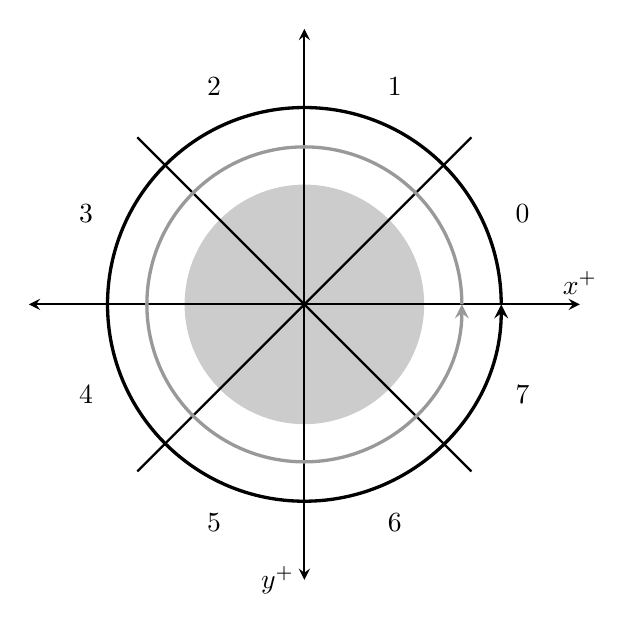
\begin{tikzpicture}[>=stealth]
			\draw [very thick, color=black!20, fill] (0,0) circle (1.5);

			%% Coordinate axes
			\draw [<->,thick] (-3.5,0) -- (3.5,0) node [above] {$x^+$};
			\draw [<->,thick] (0,3.5) -- (0,-3.5) node [left] {$y^+$};

			%% Diagonals
			\draw [thick] (0,0) +(45:-3) -- (45:3);
			\draw [thick] (0,0) +(135:-3) -- (135:3);

			%% Even arcs labels
			\foreach \x in {0,1,2,3} {
				\pgfmathmultiply{\x}{90}
				\pgfmathtruncatemacro{\alpha}{\pgfmathresult}
				\pgfmathmultiply{\x}{2}
				\pgfmathtruncatemacro{\arclabel}{\pgfmathresult}
				\path (0,0) +(22.5+\alpha:3cm) node {$\arclabel$};
			}

			%% Odd arcs labels
			\foreach \x in {0,1,2,3} {
				\pgfmathmultiply{\x}{90}
				\pgfmathtruncatemacro{\alpha}{\pgfmathresult}
				\pgfmathparse{2*\x+1}
				\pgfmathtruncatemacro{\arclabel}{\pgfmathresult}
				\path (0,0) +(67.5+\alpha:3cm) node {$\arclabel$};
			}

			%% Single arcs
			\draw [->, very thick, color=black!40] (0,0) +(0:2cm) arc (0:360:2cm);
			\draw [->, very thick] (0,0) +(0:2.5cm) arc (0:360:2.5cm);
		\end{tikzpicture}
	\end{figure}
\end{frame}

\begin{frame}{Sholl Analysis: Descriptors}
	Important descriptors
	\begin{enumerate}
		\item Sprout enumeration
		\item Average sprout length
		\item Branching factor (Shoenen Ramification Index)
		\item Critical Value
	\end{enumerate}
\end{frame}

\begin{frame}{Skeleton Reference}
	\begin{figure}
		\centering
		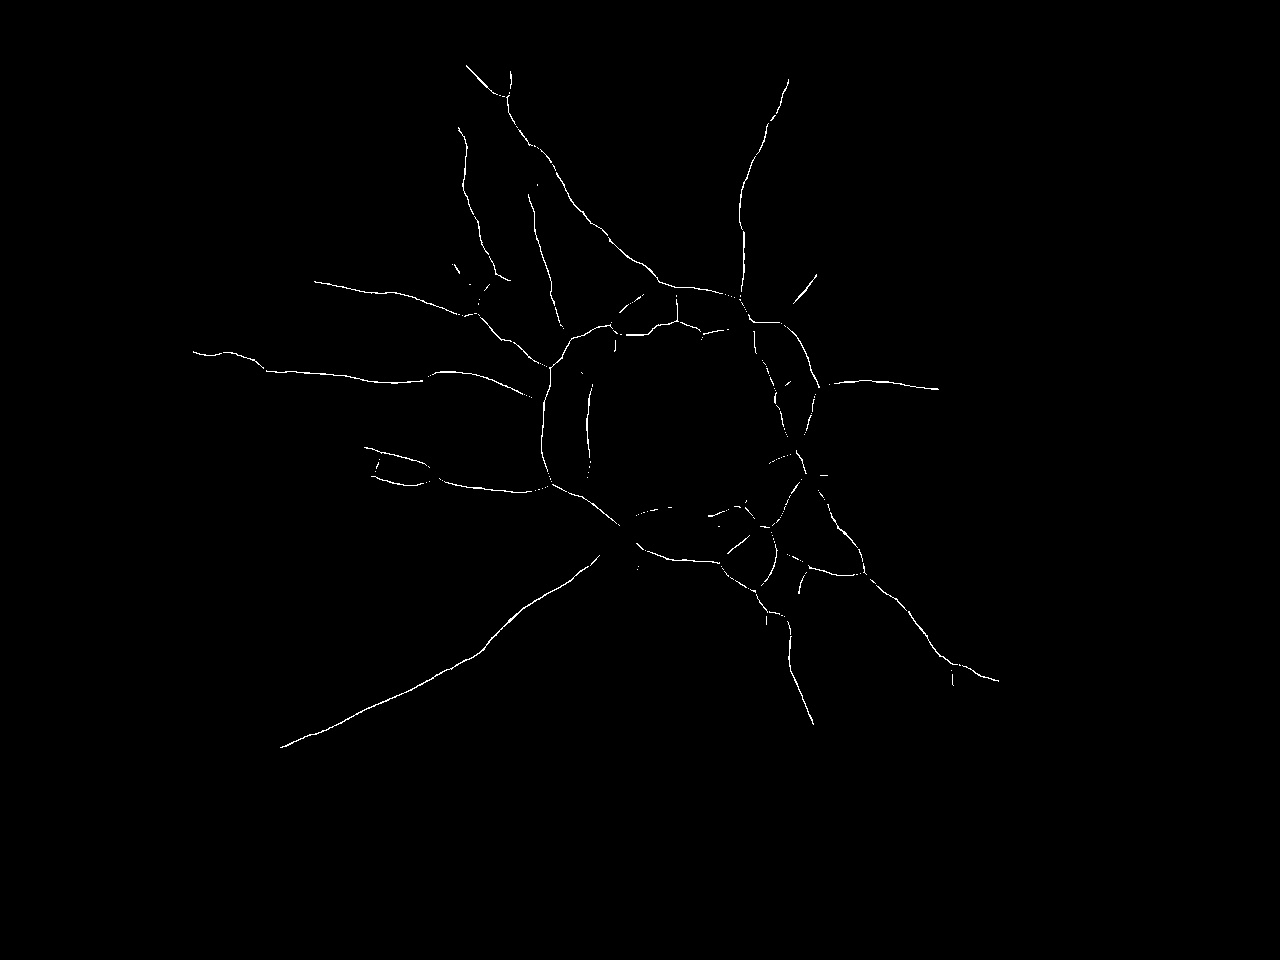
\includegraphics[width=\textwidth]{images/mono_skeletonized}
	\end{figure}
\end{frame}

\begin{frame}{Sholl Analysis: Sprout Enumeration}
	\textbf{Problem 1} Non-continuous sprouts

	\textbf{Problem 2} Bad initial radius

	\textbf{Solution} Bounded crossings integration
	\begin{itemize}
		\item Mean of $n$ crossings
		\item Median of $n$ crossings
	\end{itemize}

	\begin{figure}[h]
		\centering
		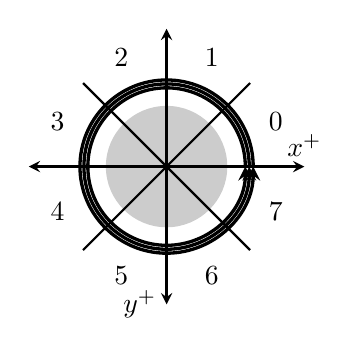
\begin{tikzpicture}[>=stealth, scale=0.5]
			\draw [very thick, color=black!20, fill] (0,0) circle (1.5);

			%% Coordinate axes
			\draw [<->,thick] (-3.5,0) -- (3.5,0) node [above] {$x^+$};
			\draw [<->,thick] (0,3.5) -- (0,-3.5) node [left] {$y^+$};

			%% Diagonals
			\draw [thick] (0,0) +(45:-3) -- (45:3);
			\draw [thick] (0,0) +(135:-3) -- (135:3);

			%% Even arcs labels
			\foreach \x in {0,1,2,3} {
				\pgfmathmultiply{\x}{90}
				\pgfmathtruncatemacro{\alpha}{\pgfmathresult}
				\pgfmathmultiply{\x}{2}
				\pgfmathtruncatemacro{\arclabel}{\pgfmathresult}
				\path (0,0) +(22.5+\alpha:3cm) node {$\arclabel$};
			}

			%% Odd arcs labels
			\foreach \x in {0,1,2,3} {
				\pgfmathmultiply{\x}{90}
				\pgfmathtruncatemacro{\alpha}{\pgfmathresult}
				\pgfmathparse{2*\x+1}
				\pgfmathtruncatemacro{\arclabel}{\pgfmathresult}
				\path (0,0) +(67.5+\alpha:3cm) node {$\arclabel$};
			}

			%% Single arcs
			\draw [->, very thick] (0,0) +(0:2cm) arc (0:360:2cm);
			\draw [->, very thick] (0,0) +(0:2.1cm) arc (0:360:2.1cm);
			\draw [->, very thick] (0,0) +(0:2.2cm) arc (0:360:2.2cm);
		\end{tikzpicture}
		\caption{Crossing integration over intervals of size $3$}
	\end{figure}
\end{frame}

\begin{frame}{Results}
	Resulting sprout counts are compared with an expert observer using 15
	images.

	\begin{equation}
		\text{RMSE} = \sqrt{\frac{1}{n}\sum^n_{i\gets 1} (\mathbf{\hat{Y}}_i - \mathbf{Y}_i)^2}
	\end{equation}

	\begin{table}
		\begin{tabular}{|l|l|}
			\hline
			\textbf{Method Variant} & RMSE \\\hline
			Median Integration Method & 1.74 \\\hline
			Ignoring isolated points & 1.79 \\\hline
			Mean Integration Method Benchmark & 1.93 \\\hline
			LIS on Large Image & 3.45 \\\hline
		\end{tabular}
		\caption{Results of Method Variants}
	\end{table}
\end{frame}

\begin{frame}{Further Work}
	\begin{enumerate}
		\item Gather results for median integration method
		\item Distinguish individual sprouts
		\item Sprout tracing similar to neuron tracing; see Meijering E.
			Neuron tracing in perspective. \emph{Cytometry A} 2010;77A:
			693–704. 
		\item Three-dimensional reconstruction using multiple image depths
	\end{enumerate}
\end{frame}

% \begin{frame}{Acknowledgements}
% 	Thanks to our mentors:
% 
% 	\begin{itemize}
% 		\item Ernie Esser
% 		\item Anna Konstorum
% 	\end{itemize}
% \end{frame}
% 
\begin{frame}
	\centering
	Thank you. Questions?
\end{frame}

\end{document}

